% The stream of frames the controller watches before it changes the resolution.
% Everything shown is real: frames from the M3FD val split, detections from the
% cached ms_fusion_seed42 run at the resolution actually in force, and decisions
% produced by replaying results/processed/sequence/controller.json over the group.
%   row A: group 496, frames 03284-03303 (20 contiguous frames, lower band shown)
%          16 frames at 576 px, then the tree reads frame 16 and sets 544 px
%   row B: group  83, frames 00801-00812 (first 12 of 24)
%          safety override after frame 6, nine frames before the window would end
%
% Black and white only: black strokes on white fills, grey reserved for secondary
% text. All type is black; grey is reserved for rules, braces and lead lines, so
% nothing relies on colour and it survives photocopying and greyscale print.
%
% Strip geometry: a thumbnail is 400 px wide with a 26 px gap, so at an image width
% of 16.20 cm the pitch is 16.20*426/8494 = 0.81249 cm and a thumbnail is 0.76309 cm
% wide.  Frame i has centre 3.10 + (i-1)*0.81249 + 0.38155.  Row A thumbnails are
% cropped to the lower band (aspect 0.575), row B thumbnails are whole (0.75).
%
% Layout contract: a text line is 0.388 high and a box adds 0.28 of padding, so an
% n-line box is 0.388n + 0.28. Every label keeps >= 0.25 clear of every box.
\documentclass[tikz,border=0pt]{standalone}
\usepackage[T1]{fontenc}
\usepackage{graphicx}
\usepackage{tgtermes}
\usetikzlibrary{arrows.meta,calc,positioning}

\newcommand{\bd}[1]{{\fontsize{13}{15}\selectfont #1}}
\newcommand{\bt}[1]{{\fontsize{8.4}{9.6}\selectfont #1}}
\newcommand{\bn}[1]{{\fontsize{7.5}{9}\selectfont #1}}
\newcommand{\bs}[1]{{\fontsize{7}{8.2}\selectfont\textcolor{Ink}{#1}}}
\newcommand{\dt}{\,\textperiodcentered\,}

\definecolor{Ink}{gray}{0.05}
\definecolor{Muted}{gray}{0.32}
\definecolor{Rule}{gray}{0.70}
\definecolor{Fill}{gray}{0.93}

\tikzset{
  base/.style={rounded corners=2pt,align=center,text=Ink,fill=white,
    inner xsep=5pt,inner ysep=4pt},
  read/.style={base,draw=Ink,line width=0.7pt},
  act/.style={base,draw=Ink,line width=1.3pt,fill=Fill},
  head/.style={font=\fontsize{9}{11}\selectfont,text=Ink,anchor=west},
  note/.style={font=\fontsize{7}{8.2}\selectfont,text=Ink,align=center},
  noteL/.style={note,align=left},
  flow/.style={-{Latex[length=2.3mm,width=1.4mm]},line width=0.9pt,draw=Ink},
  thin/.style={line width=0.5pt,draw=Ink},
  lead/.style={line width=0.45pt,draw=Muted,densely dashed},
  stepln/.style={line width=1.3pt,draw=Ink},
  gridln/.style={line width=0.4pt,draw=Rule,densely dotted},
  axisln/.style={line width=0.6pt,draw=Ink},
  brace/.style={line width=0.6pt,draw=Muted},
  tick/.style={line width=0.5pt,draw=Rule},
}

% centre x of frame #1 in either strip
\newcommand{\cx}[1]{3.10 + (#1-1)*0.81249 + 0.38155}

\begin{document}
\begin{tikzpicture}[x=1cm,y=1cm]
  \path[use as bounding box] (0,0.10) rectangle (20.60,12.30);
  \fill[white] (0,0.10) rectangle (20.60,12.30);

  % ================================================================== title
  \node[head] at (0.40,11.92)
    {\bd{The controller watches the stream, and only then changes the size.}};
  \node[note,anchor=east] at (20.20,11.92)
    {M3FD val split \dt{} one resolution per frame \dt{} no probe pass};
  \draw[Rule,line width=0.5pt] (0.40,11.60) -- (20.20,11.60);

  % ============================================================ row A: head
  \node[head] at (0.40,11.22)
    {A\dt{} the ordinary case: sixteen frames go by, then the size drops};
  \node[note,anchor=east] at (20.20,11.22)
    {group 496 \dt{} frames 03284--03303 \dt{} visible channel, lower band};

  % ---------------------------------------------------------- row A: strip
  \draw[brace] (3.10,10.52) -- (3.10,10.66) -- (16.04,10.66) -- (16.04,10.52);
  \draw[brace] (16.11,10.52) -- (16.11,10.66) -- (19.30,10.66) -- (19.30,10.52);
  \node[note,anchor=south] at (9.57,10.70)
    {16 frames at 576\,px \dt{} every one is summarised, not one of them changes the size};
  \node[note,anchor=south] at (17.70,10.70) {held at 544\,px};

  \node[anchor=north west,inner sep=0pt] at (3.10,10.42)
    {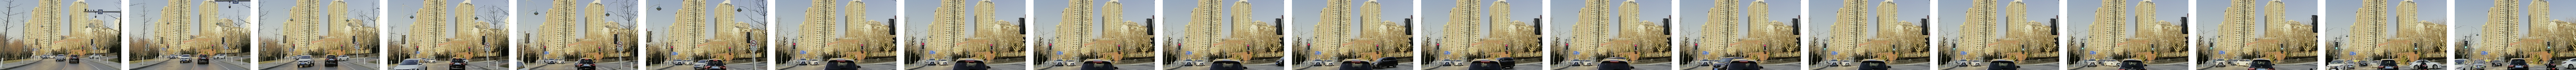
\includegraphics[width=16.20cm]{assets/stream_a_vis.png}};
  \draw[tick] (3.10,10.42) rectangle (19.30,9.982);

  \foreach \i/\lab in {1/1, 8/8, 16/16, 17/17, 20/20}
    \node[note,anchor=north] at ({\cx{\i}},9.90) {\lab};
  \node[note,anchor=east] at (2.95,9.76) {frame};

  % the decision instant
  \draw[lead] (16.075,9.982) -- (16.075,8.90);
  \node[note,anchor=east] at (15.95,9.30) {the tree fires once, here};
  \fill[Ink] (16.075,8.48) circle (0.055);

  % ---------------------------------------------------- row A: resolution
  \foreach \y in {7.64, 8.06, 8.48, 8.90} \draw[gridln] (3.10,\y) -- (19.30,\y);
  \foreach \y/\lab in {7.64/480, 8.06/544, 8.48/576, 8.90/640}
    \node[note,anchor=east] at (2.95,\y) {\lab};
  \draw[axisln] (3.10,7.44) -- (19.30,7.44);
  \draw[stepln] (3.10,8.48) -- (16.075,8.48) -- (16.075,8.06) -- (19.30,8.06);
  \node[note,anchor=south] at (9.57,8.55) {576\,px};
  \node[note,anchor=south] at (17.70,8.13) {544\,px};
  \node[note,rotate=90] at (1.50,8.27) {the size the detector runs at};

  % ------------------------------------------------------- row A: callout
  \node[anchor=north west,inner sep=0pt] at (3.10,7.19)
    {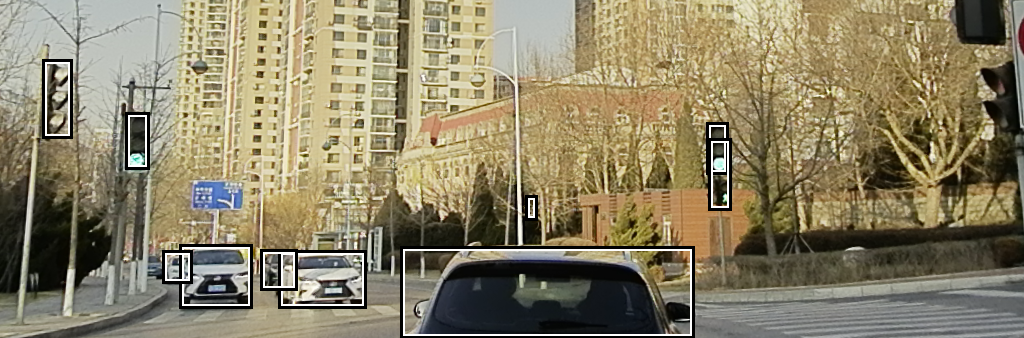
\includegraphics[width=5.00cm]{assets/stream_a_key.png}};
  \draw[tick] (3.10,7.19) rectangle (8.10,5.54);
  \node[noteL,anchor=north west] at (3.10,5.40)
    {frame 16 \dt{} 03299 \dt{} the same lower band, enlarged\\
     boxes: what the detector had \emph{already} returned at 576\,px};

  \draw[flow] (8.25,6.365) -- (8.80,6.365);
  \node[read,anchor=west,align=center] at (8.80,6.365)
    {\bt{what the tree reads from it}\\[1pt]
     \bn{10 candidates at conf.\ $\geq$ 0.10 \dt{} none of them a \textit{People}}\\
     \bn{mean conf.\ of the top 10 = 0.62 \dt{} median box 1\,960\,px$^2$}\\
     \bn{no \textit{People} $\to$ 0.62 $>$ 0.24 $\to$ 10 $\leq$ 12 candidates}};

  \draw[flow] (15.55,6.365) -- (16.10,6.365);
  \node[act,anchor=west,align=center] at (16.10,6.365)
    {\bd{544\,px}\\[1pt]
     \bn{held for the}\\ \bn{next 16 frames}};

  \node[noteL,anchor=north west] at (8.80,5.40)
    {the summary is recomputed after every frame, and costs no second inference pass ---\\
     it is a statistic of boxes the detector has already returned --- but only the newest\\
     one, the summary of frame 16, is ever read.};

  \draw[Rule,line width=0.4pt] (0.40,4.10) -- (20.20,4.10);

  % ============================================================ row B: head
  \node[head] at (0.40,3.80)
    {B\dt{} the exception: a small pedestrian appears and the window is abandoned};
  \node[note,anchor=east] at (20.20,3.80)
    {group 83 \dt{} frames 00801--00812 \dt{} visible channel};

  % ---------------------------------------------------------- row B: strip
  \draw[brace] (3.10,3.02) -- (3.10,3.16) -- (7.91,3.16) -- (7.91,3.02);
  \draw[brace] (7.99,3.02) -- (7.99,3.16) -- (12.80,3.16) -- (12.80,3.02);
  \node[note,anchor=south] at (5.50,3.20) {6 frames at 576\,px};
  \node[note,anchor=south] at (10.40,3.20)
    {640\,px, nine frames before the window would have ended};

  \node[anchor=north west,inner sep=0pt] at (3.10,2.92)
    {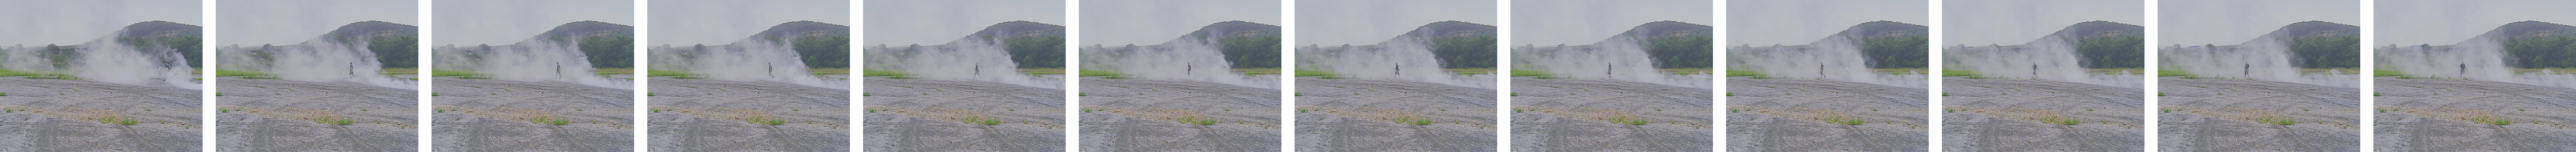
\includegraphics[width=9.70cm]{assets/stream_b_vis.png}};
  \draw[tick] (3.10,2.92) rectangle (12.80,2.348);

  \foreach \i/\lab in {1/1, 6/6, 7/7, 12/12}
    \node[note,anchor=north] at ({\cx{\i}},2.27) {\lab};
  \node[note,anchor=east] at (2.95,2.13) {frame};

  % ---------------------------------------------------- row B: resolution
  \foreach \y in {0.44, 0.86, 1.28, 1.70} \draw[gridln] (3.10,\y) -- (12.80,\y);
  \foreach \y/\lab in {0.44/480, 0.86/544, 1.28/576, 1.70/640}
    \node[note,anchor=east] at (2.95,\y) {\lab};
  \draw[axisln] (3.10,0.24) -- (12.80,0.24);
  \draw[lead] (7.950,2.348) -- (7.950,1.70);
  \draw[stepln] (3.10,1.28) -- (7.950,1.28) -- (7.950,1.70) -- (12.80,1.70);
  \node[note,anchor=north] at (5.50,1.22) {576\,px};
  \node[note,anchor=north] at (10.40,1.64) {640\,px};
  \node[note,anchor=west] at (8.10,1.49) {\bn{override}};

  % ------------------------------------------------------- row B: callout
  \node[anchor=north west,inner sep=0pt] at (13.30,2.92)
    {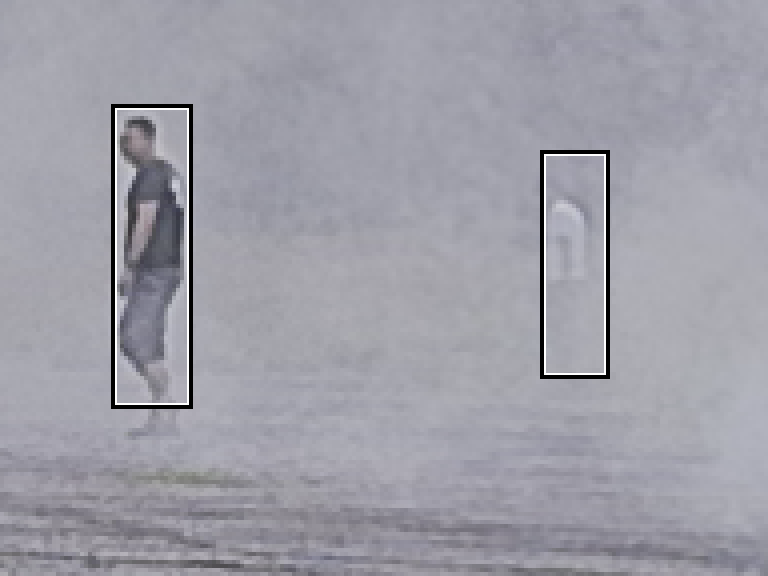
\includegraphics[width=2.00cm]{assets/stream_b_key.png}};
  \draw[tick] (13.30,2.92) rectangle (15.30,1.42);
  \node[noteL,anchor=north west] at (13.30,1.28) {frame 6 \dt{} 00806 \dt{} $4\times$ zoom};

  \draw[flow] (15.45,2.17) -- (15.95,2.17);
  \node[read,anchor=west,align=center] at (15.95,2.17)
    {\bt{the one rule that cannot wait}\\[1pt]
     \bn{a second pedestrian, 981\,px$^2$,}\\
     \bn{under the $32^2 = 1\,024$\,px$^2$ line}\\
     \bn{$\to$ 640\,px now, window restarts}};
\end{tikzpicture}
\end{document}
